\documentclass[../../spr.tex]{subfiles}

\begin{document}

\section{Testy}
\subsection{Opis metod testowania (np. testy manualne i automatyczne)}

W projekcie zastosowano automatyczne testy integracyjne warstwy kontrolerów w aplikacji Spring Boot.
Testy uruchamiane są na pełnym kontekście aplikacji,
co pozwala na weryfikację poprawności działania endpointów HTTP wraz z rzeczywistą logiką biznesową.
W celu zapewnienia izolacji testów od zewnętrznych systemów, komponenty komunikujące się z
usługami zewnętrznymi są mockowane, natomiast pozostałe serwisy odpowiedzialne za logikę biznesową
działają rzeczywiście. Takie podejście umożliwia sprawdzenie zarówno poprawności odpowiedzi HTTP,
walidacji danych, jak i integracji kontrolerów z warstwą serwisów.
Testy pozwalają na wykrywanie błędów na poziomie integracji, jednocześnie gwarantując stabilność
i powtarzalność testów poprzez eliminację zależności od zewnętrznych systemów.


\subsection{Wyniki testów, napotkane błędy oraz zastosowane rozwiązania}

Przeprowadzone testy integracyjne potwierdziły poprawność działania endpointów (zob. \ref{fig:test-results}).  
Testy typu \texttt{GET} na endpointach takich jak \texttt{/hall-types}, \texttt{/memberships}, \texttt{/membership-types} oraz \texttt{/workout-sessions} zwracały kod odpowiedzi \texttt{200} oraz listy rekordów, co świadczy o poprawnej implementacji operacji pobierania danych.
Testy typu \texttt{POST}, takie jak tworzenie nowych sesji treningowych czy członkostw, zwracały kod \texttt{201}, potwierdzając sukces operacji tworzenia rekordów.
Operacje \texttt{PATCH}, np. aktualizacja danych członkostwa, również działały poprawnie – serwer zwracał kod \texttt{200} oraz zaktualizowane dane.
Testy typu \texttt{DELETE}, np. usuwanie uczestników lub ćwiczeń z sesji treningowych, kończyły się kodem \texttt{204}, a następnie testy \texttt{GET} potwierdzały, że rekordy zostały skutecznie usunięte.
Testy scenariuszy negatywnych, takich jak próba pobrania nieistniejących zasobów lub wysłanie niepoprawnych danych, skutkowały odpowiednimi kodami błędów: \texttt{404} oraz \texttt{400}, co było zgodne z założeniami.
Ogólnie testy wykazały wysoką stabilność API. W przypadku wystąpienia jakichkolwiek krytycznych błędów, system CI nie generowałby artefaktów, a testy nie przechodziłyby poprawnie – co nie miało miejsca.

\begin{figure}[H]
  \centering
  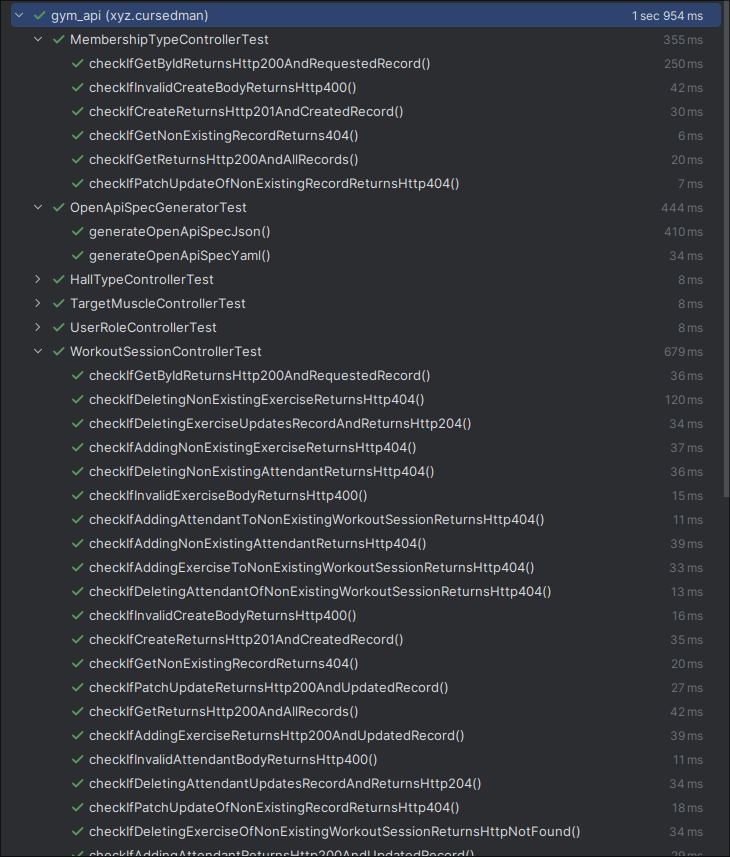
\includegraphics[width=\textwidth]{tests.png}
  \caption{Wyniki testów integracyjnych}
  \label{fig:test-results}
\end{figure}
\end{document}